\section{What kind of solver is CP-SAT?}

CP-SAT solves \textbf{constraint optimization problems over integer variables}.
You declare integer and Boolean variables with finite domains, post constraints
that link them, and optionally add a linear objective. The solver then finds an
assignment that satisfies every constraint and optimizes the objective, or proves
that none exists. That is the complete-search promise. Under a time or resource
limit, CP-SAT may instead return the best solution and bound it has found so far,
or report that the status is still unknown.

There are other solvers with that promise, but what makes CP-SAT distinctive
is its lineage. It fuses two solver traditions that historically lived apart:

\begin{itemize}
  \item \textbf{Constraint Programming (CP)}, whose strength is
  \emph{propagation}: rich, problem-specific reasoning that prunes domains
  (``if these three tasks cannot overlap and two are already scheduled here, the
  third cannot start before time 12''). \Cref{fig:sudoku-propagation} shows the
  idea on a Sudoku.
  \item \textbf{Conflict-Driven Clause Learning (CDCL) SAT}, whose strength is
  \emph{learning from failure}: whenever search reaches a dead end, it distills
  the failure into a reusable rule, a ``nogood,'' so that it never repeats the
  same mistake (\cref{fig:sudoku-conflict}).
\end{itemize}

A one-line example shows what propagation means. Suppose two variables
$x, y \in \{0,1,\dots,5\}$ are tied by the constraint $x + y \le 5$, and the
search guesses $x \ge 4$. The constraint immediately forces $y \le 1$, so the
solver shrinks $y$'s domain to $\{0,1\}$ with no further guessing. That shrinking
is \textbf{propagation}: a constraint ruling out the values a variable can no
longer take. The piece of code that does it for one constraint is its
\textbf{propagator}. \Cref{fig:sudoku-propagation} shows the same mechanism at
Sudoku scale, where one forced value cascades into many.

\begin{figure}[tb]
\centering
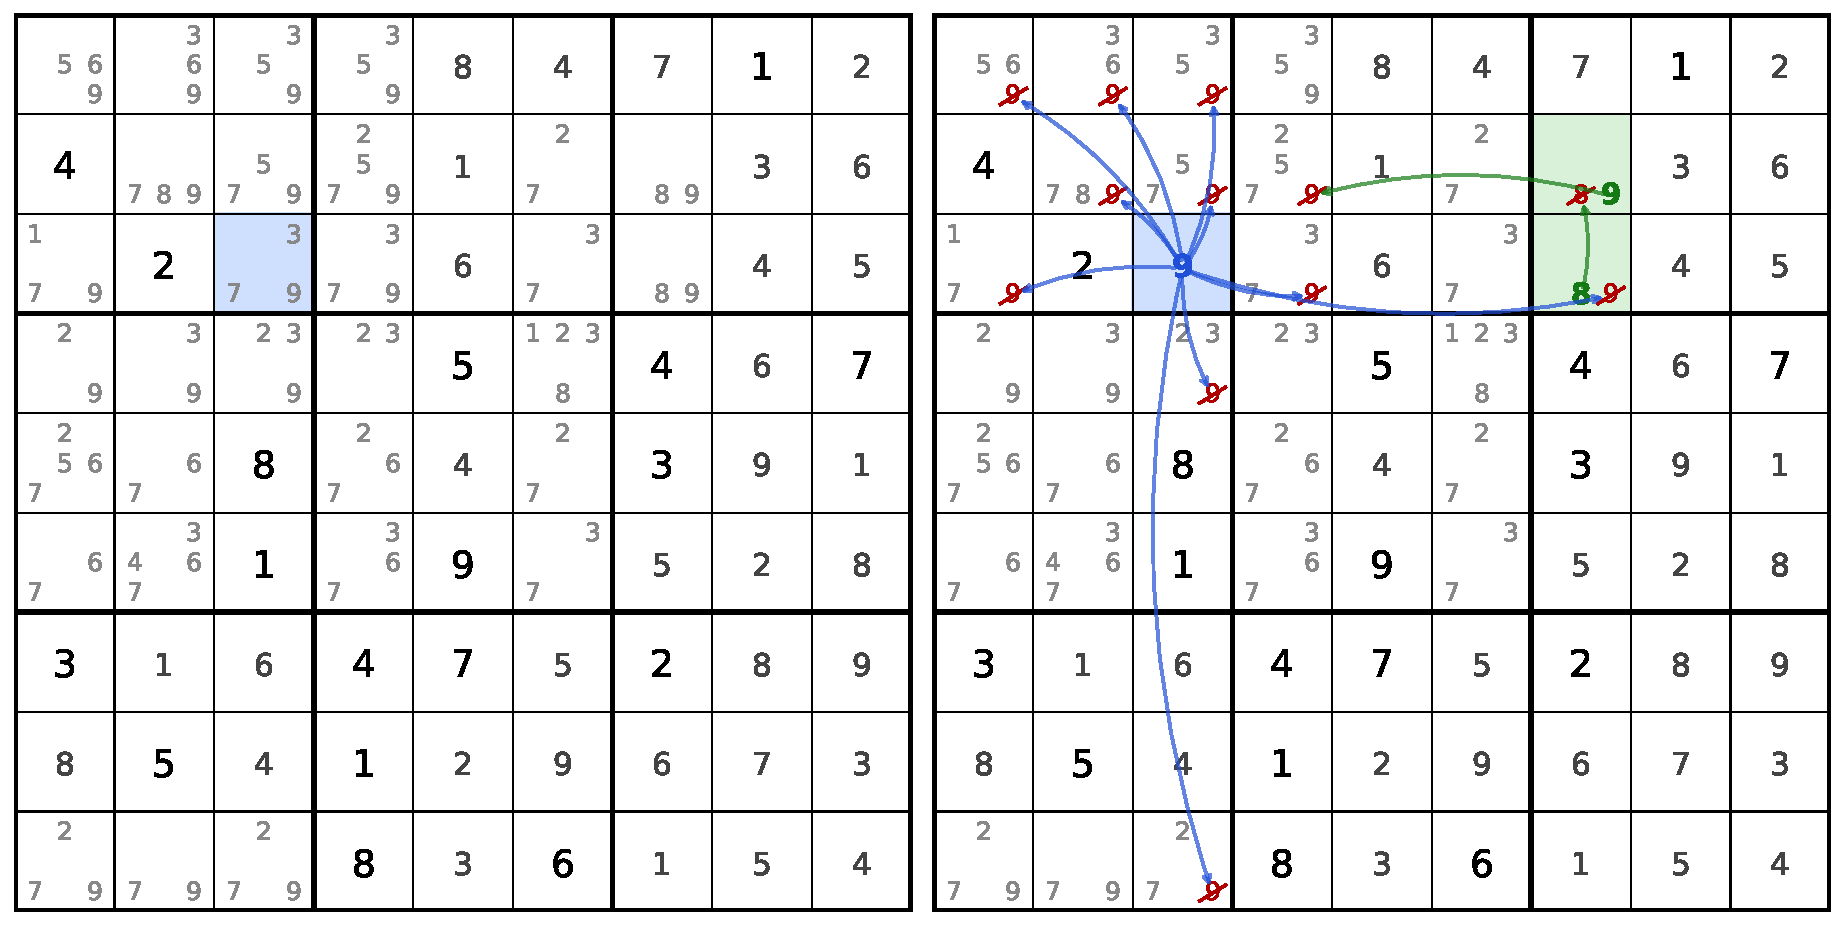
\includegraphics[width=\linewidth]{figures/sudoku/propagation_sudoku.pdf}
\caption{\textbf{Propagation} on a Sudoku: each cell is a variable, the
\emph{all-different} constraints on rows, columns, and boxes are the propagators,
and the small pencil marks are each cell's remaining candidates. \textbf{Left:}
the givens propagated as far as they go; every empty cell still has several
candidates and none is forced, so search must guess. \textbf{Right:} we guess a
\textbf{blue} value; the propagators strike it from every peer (blue arrows), one
peer loses its last alternative and is forced, which forces a \textbf{green}
value, and the deductions cascade to a new fixed point with no further guessing.}
\label{fig:sudoku-propagation}
\end{figure}

\begin{figure}[tb]
\centering
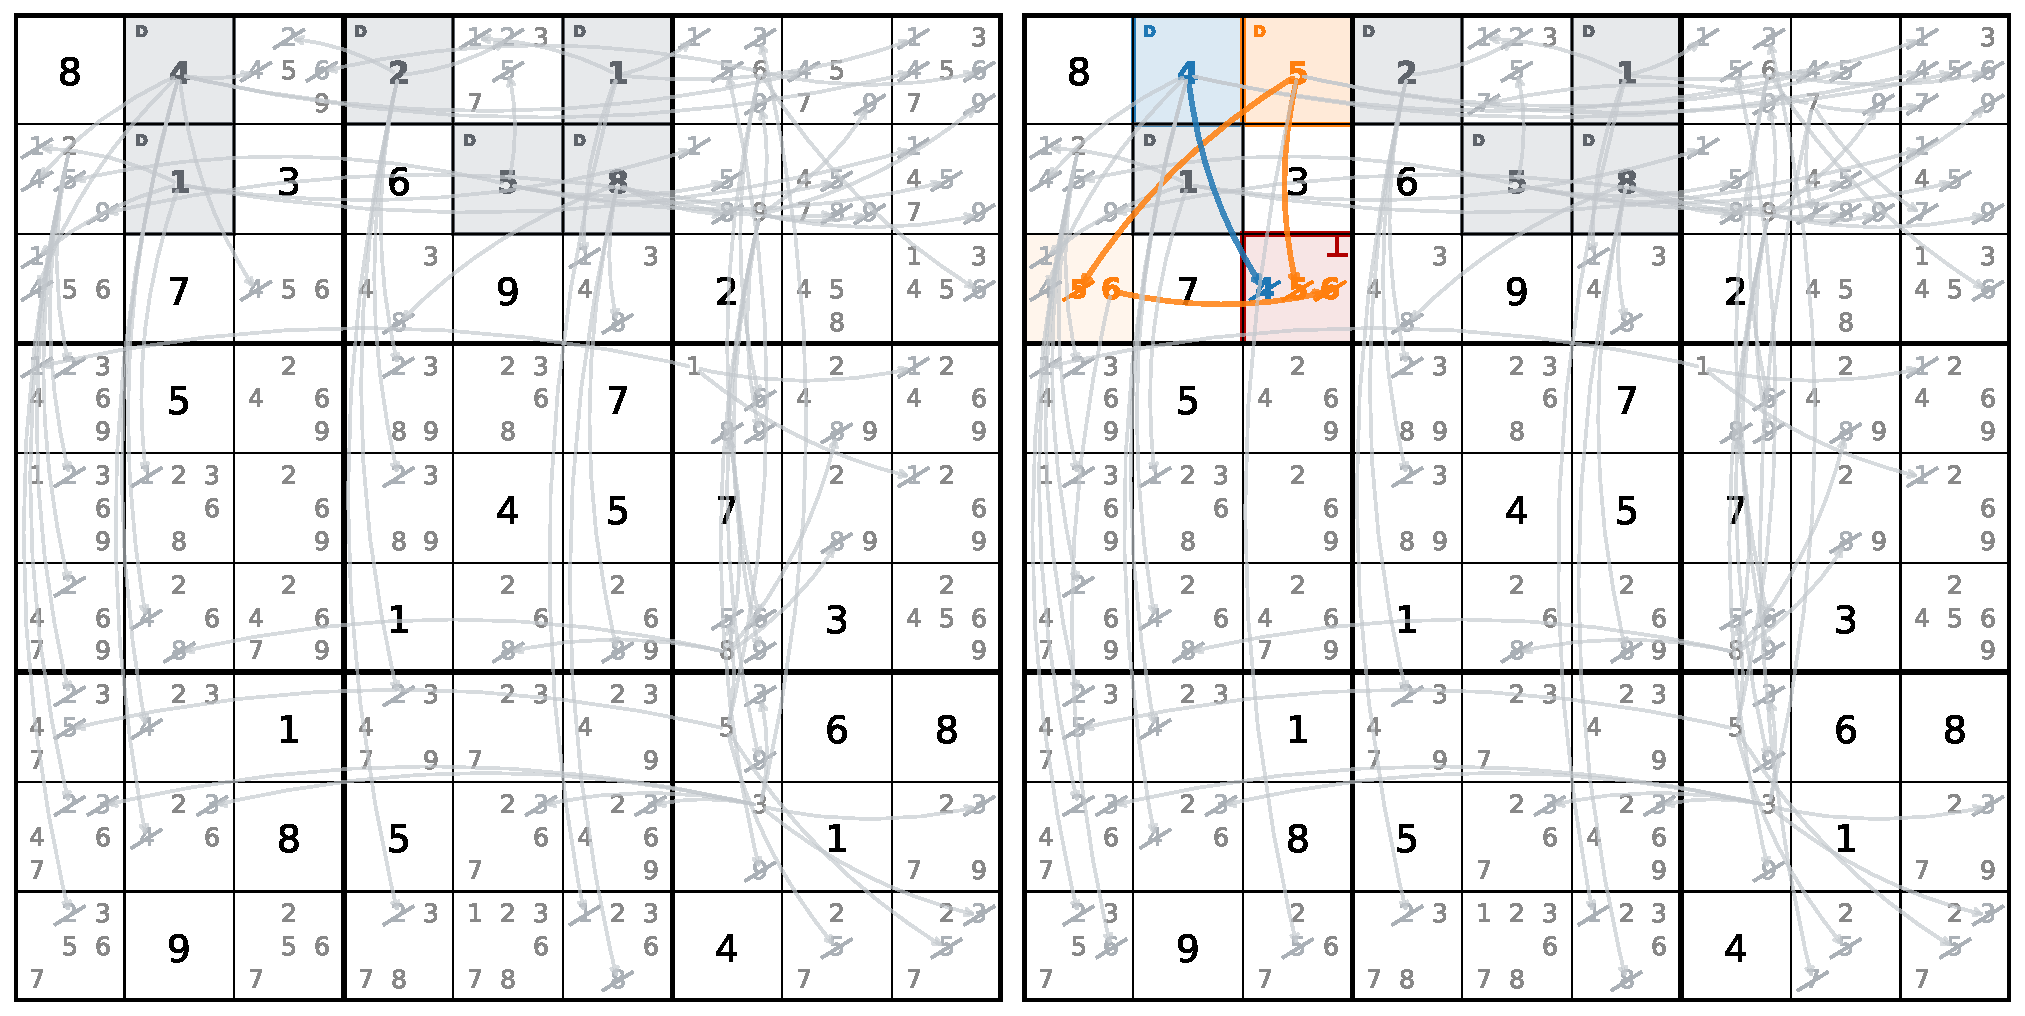
\includegraphics[width=\linewidth]{figures/sudoku/conflict_sudoku.pdf}
\caption{\textbf{Conflict analysis} on a Sudoku. \textbf{Left:} six guesses (grey,
tagged $D$) have been placed and propagated, and nothing has failed yet.
\textbf{Right:} a seventh guess (\textbf{orange}) propagates and empties one cell's
domain (\textbf{red}, $\bot$): a \textbf{conflict}. Tracing the struck candidates
backward shows that only \emph{two} of the seven guesses are jointly to blame (the
orange one and a \textbf{blue} one); the other five never touched this cell. From
these two the solver learns a \textbf{SAT clause} (a nogood) that bars the
combination forever, then backjumps past the five irrelevant guesses instead of
just undoing the last one.}
\label{fig:sudoku-conflict}
\end{figure}

Classic CP search is good at pruning but tends to be amnesiac: it backtracks and
forgets why it failed. Classic SAT learns effectively but only speaks in Boolean
clauses and cannot compactly express arithmetic relations among integer variables.
CP-SAT's central idea,
\textbf{lazy clause generation}, combines the two: CP-style propagators perform
the pruning, but every pruning step is justified by a reason from which the CDCL
engine can learn. The result is a CP solver with a SAT solver's memory.
% Source (developers' own framing of the lineage): the CP-SAT developers trace
% the architecture to Peter Stuckey's "Search is Dead" (CP 2013) and the lazy
% clause generation line of work, deliberately discarding classic CP search
% machinery in favor of a SAT core that learns.
\begin{platypusbook}[htb]
The developers trace CP-SAT's lineage directly to the lazy-clause-generation work of
the late 2000s, notably Peter Stuckey's pointed ``search is dead'' framing, and
built CP-SAT by deliberately discarding the classic CP search machinery in favor
of a learning SAT core. For the fuller story, see Stuckey's
\href{https://youtu.be/lxiCHRFNgno}{talk on lazy clause generation}~\cite{stuckey2014lcg}
and the CP-SAT developers' own overview talks~\cite{perron2020cpaior,perron2024scheduling,perron-ewo-ortools}.
\end{platypusbook}

Two further ingredients complete the picture. The rest of this text treats them
as accelerators bolted onto the core (\cref{part:faster}, \emph{Going faster}),
but they are central to what CP-SAT \emph{is}, and any honest description should
name them up front.

\begin{itemize}
  \item \textbf{A linear-programming relaxation, run as a propagator.} Alongside
  the search, LP-enabled CP-SAT workers maintain a continuous LP relaxation of
  the model and re-solve it with the dual simplex as a high-cost propagator,
  typically after cheaper propagation has stalled. The LP relaxation feeds back
  global numeric bounds, reduced-cost reasoning, and cutting planes
  (\cref{sec:lp,sec:cuts}). This creates the bridge to the
  \textbf{MIP} (mixed-integer programming) world of branch-and-cut: a third
  solver tradition folded in beside CP and SAT, and the reason CP-SAT holds its
  own on problems with strong linear structure where pure propagation is weak.
  \item \textbf{A parallel portfolio, not a single search.} Given several
  threads, CP-SAT does not partition one tree. It runs a \textbf{portfolio} of
  workers instead, most of them differently configured copies of the same core
  (some LP-heavy, some pure CP/SAT, some core-guided on the objective), together
  with a set of primal heuristics. These
  workers attack the whole problem at once and continuously share the clauses
  and bounds they learn (\cref{sec:portfolio}).
\end{itemize}

So the compact answer to ``what is CP-SAT?'' is: a CDCL learning core, fed by CP
propagation \emph{and} an LP relaxation, diversified across a cooperating
portfolio.
